\paragraph{}
Le projet du groupe 3\footnote{L'équipe composée de Louis Randriamora Andriantsiory, Kolawole Abdoulaye et Rudy Itunime Masala} consiste en la gestion d'une ludothèque, un centre de prêt de jeux en tout genre; jeux vidéos, jeux de société ou autres jouets.
\paragraph{}
Selon les spécificités décidées par le groupe 3, un jeu doit avoir un nom, un statut de disponibilité et un fabricant, quel que soit son type.\\
Certains types de jeux spécifiques ont des caractéristiques propres, ce qui entraîne l'utilisation de l'héritage, décrite au point \ref{subsection:structure}.
\paragraph{}
L'application devrait permettre au gérant de s'identifier, et de gérer la ludothèque; ajouter des jeux, faire des recherches, obtenir une liste de prêts, etc. \\
Elle devrait également permettre aux adhérents de faire des recherches de jeux, voyant lesquels sont disponibles ou non et de déclarer un emprunt.
\paragraph{}
L'application, codée en java, utilise les concepts de programmation orientée objet. La structure du programme est donc composée de classes représentant les différents objets ou acteurs intervenant. 

\subsection{Structure}
    \label{subsection:structure}
    \subsubsection{Classes et fonctionnalités}
        \begin{figure*}[h!]
                \centering
                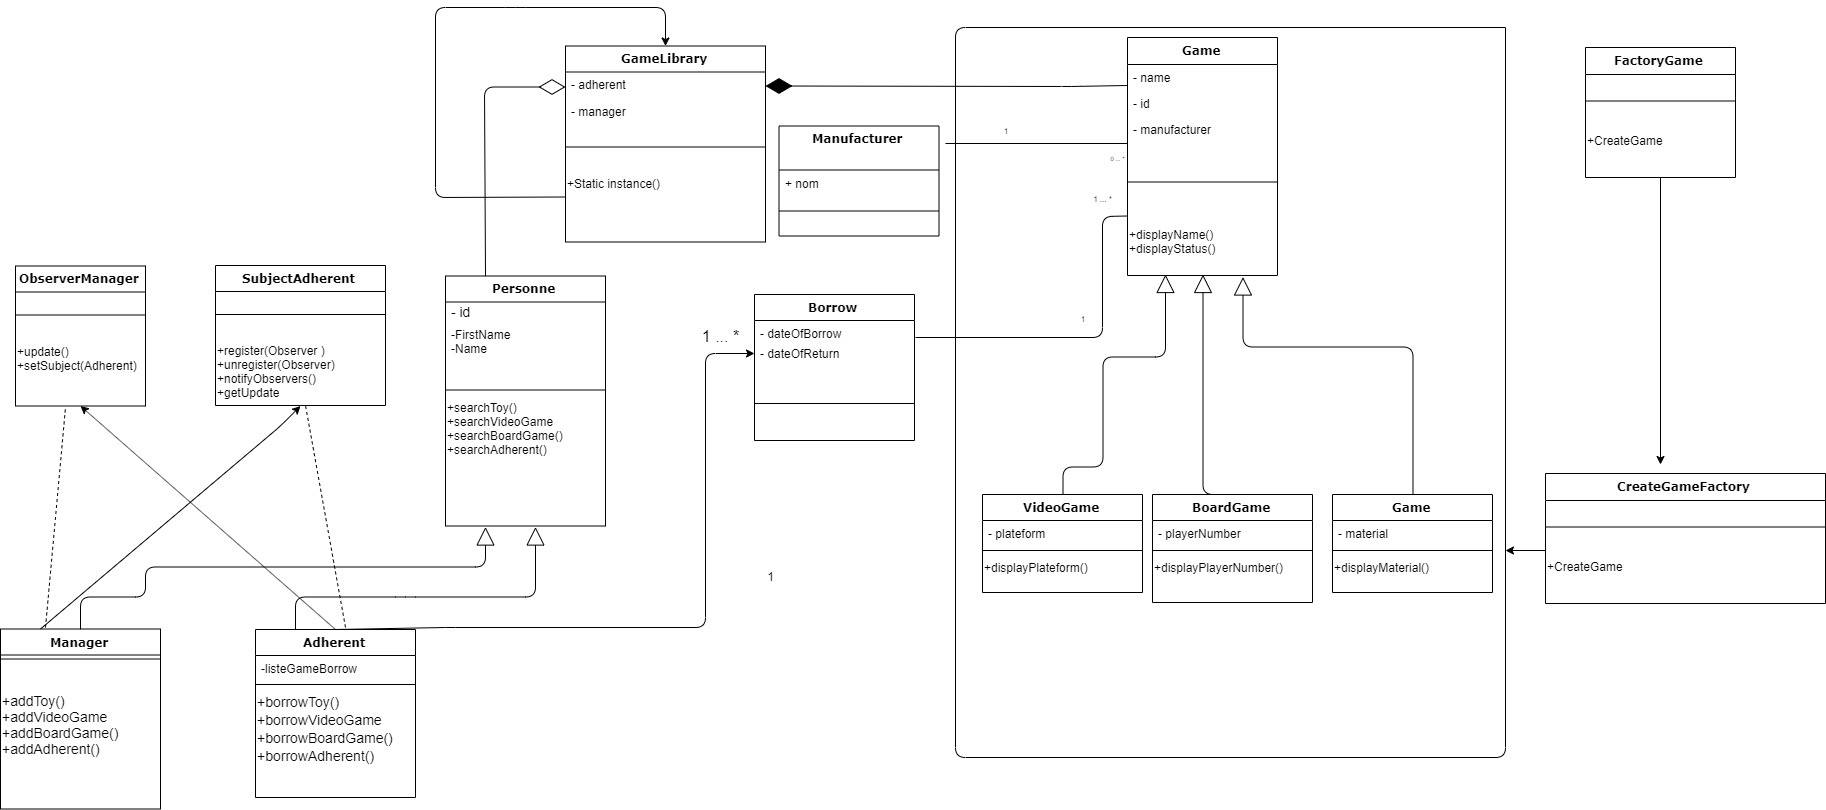
\includegraphics[width=\textwidth,center]{Figures/Class_Diagram.jpg}
                \caption{Diagramme de classe}
                \label{fig:classDiagram_old}
            \end{figure*}
        \newpage
        Le diagramme de classe en figure \ref{fig:classDiagram_old} représente la structure du projet que nous avons auditionné, et est repris en annexe en figure \ref{fig:annexe:classDiagram_old} pour plus de lisibilité.  
        \paragraph{}
        On observe sur ce diagramme que la première équipe de dévelopement avait créé une classe Game, de laquelle héritaient 3 sous-classes Game, BoardGame et VideoGame. Le diagramme ne semble pas à jour\footnote{Par rapport à l'état dans lequel nous avons récupéré le projet}, puisque la classe-fille Game a été remplacée par une classe Toy. 
        La super-classe Game est une classe abstraite et ne peut pas être implémentée.
        \paragraph{}
        4 différentes interfaces étaient présentes dans le code et ne sont pas reprises dans le diagramme de classe\footnote{AdherentFacade, ObserverManager, SubjectAdherent et UserFacade}. Ces interfaces sont des parties de design patterns qui seront décrits en sous-section \ref{subsubsection:design} : Design.
        \paragraph{}
        En outre, les relations entre les classes ne sont pas toutes claires, comme celle entre la classe Borrow et la classe Game, et celle entre la classe Manufacturer et la classe Game. Les aggrégations et compositions sont quant à elles plus claires; une GameLibrary est composée de Game, et a des Personne\footnote{Noté en français dans le diagramme de classe}, soit Manager soit Adherent.  
    \subsubsection{Design patterns}
        \label{subsubsection:design}
        \paragraph{}
        Le groupe 3 a choisi d'utiliser plusieurs designs patterns : l'observer, le facade, et le factory. \\
        Le design pattern observateur est utilisé pour envoyer des signaux à des modules, les observateurs. En cas de notification, les observateurs peuvent effectuer l'action adéquate en fonction des informations reçues. En pratique, le groupe 3 a implémenté l'observateur mais ne l'utilise pas. \\
        En effet, les interfaces ObserverManager et SubjectAdherent existent et présentent des méthodes typiques du design pattern (notifyObserver chez le subjectAdherent, setSubject qui est l'action de l'observateur), mais ne sont jamais utilisées et leurs méthodes jamais appelées. \\
        Le design pattern observer suit typiquement la structure représentée en figure \ref{fig:observer}.
        \begin{figure*}[h!]
                \centering
                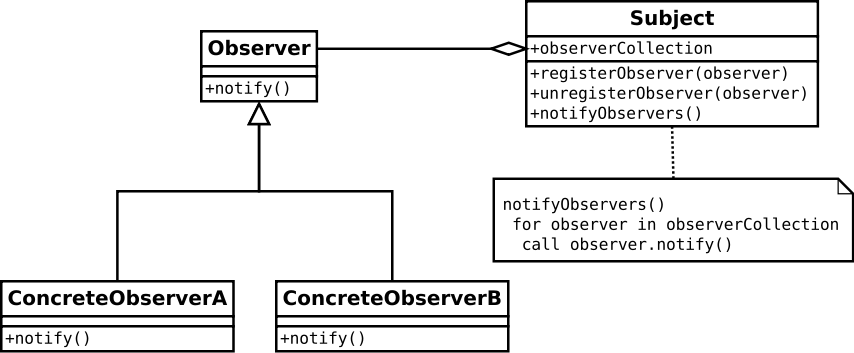
\includegraphics[width=\textwidth,center]{Figures/Observer.png}
                \caption{Design pattern observer}
                \label{fig:observer}
        \end{figure*}
        \newpage{}
        \paragraph{}
        Le design pattern factory permet d'instancier des objets héritant d'une classe abstraite, et donc d'instancier des objets dont la classe exacte est inconnue. \\
        Le factory est ici utilisé pour instancier des jeux, quel que soit leur types. Cependant, l'implémentation de ce design pattern n'était pas terminée et nous avons dû y apporter de nombreuses modifications. 
        \paragraph{}
        Le design pattern facade doit cacher une interface et conception complexe, en proposant au développeur ou utilisateur une interface plus simple et générique.\\
        Le UserFacadeImpl, qui implémentait une interface UserFacade\footnote{L'interface oblige le développeur à implémenter une méthode managerMenu, et une méthode adherentMenu, méthodes dont le rôle est de gérer un menu utilisateur}. A nouveau, de nombreuses modifications ont été apportées à la classe UserFacadeImpl.
        
    \subsubsection{Paradigmes}
        Le projet de ludothèque répondant à un problème concret, représentant une situation du monde réel, et comprenant des représentations d'objets physiques, la programmation orientée objet semble tout indiquée. \\ 
        Il existe une multitude de langages de programmation orientée objet; l'utilisation de Java est pertinente puisque c'est un langage de POO pour lequel de nombreux outils de qualités et d'intégration existent\footnote{C'est bien sûr le cas d'autres langages, mais la programmation Java faisait partie des exigences du client, le professeur}. 
        \paragraph{}
        Justifions la structure du projet et son design en fonction du problème auquel il répond.
        \newpage
        Le design pattern observateur semble servir à notifier le manager lorsqu'un adhérent s'enregistre, requièrant une action de ce dernier, probablement mettre à jour la base de données avec les informations de l'adhérent. Il est malheureusement difficile d'en être certain puisque le design pattern n'était pas utilisé dans le projet. 
        \paragraph{}
        La classe GameFactory permet de créer une instance de jeu, quel que soit son sous-type. La méthode principale (et unique) de cette classe est createGame, qui reçoit en paramètre les informations nécessaires à l'instanciation du jeu. Cette méthode ne respecte pas l'extensibilité, puisque si un développeur souhaite ajouter un autre type de jeu, il devra obligatoirement modifier la méthode createGame également. 
        \paragraph{}
        Le rôle de la classe UserFacadeImpl est de gérer l'interface utilisateur du programme. Puisque ce programme est exclusivement exécuté en terminal, sans interface graphique, cette classe appelle principalement des fonctions et classes terminales telles que println ou Scanner, qui alourdissent la lecture du code; il est donc intéressant de les placer dans une classe à part et non directement dans le main, ou dans une autre classe. 
        
\subsection{Critères de qualité}
    \paragraph{}
    La première équipe de développement a déclaré vouloir respecter les critères de qualité suivants : le projet doit être maintenable, respecter le concept d'intégrité, être "simple" et être extensible.\\ Le critère de simplicité est décrit par le groupe\footnote{Voir page 3 du rapport préliminaire du groupe} comme la facilité à comprendre la structure du projet et la logique des algorithmes et du code. 
    \paragraph{}
    La maintenabilité d'un logiciel décrit l'effort nécessaire pour comprendre, corriger ou modifier ce logiciel pour un développeur, extérieur au projet ou non. \\
    Le rapport préliminaire du groupe 3 indique qu'ils respectent ce critère par l'utilisation de la programmation orientée objet; il s'agit d'une erreur, puisque l'utilisation de la POO n'est pas garante de maintenabilité en soit.
    \paragraph{}
    Le critère de simplicité découle en réalité de celui de maintenabilité, et n'est donc pas un critère de qualité à part entière.  
    \paragraph{}
    L'intégrité, que le groupe déclare respecter à l'aide de tests unitaires, est la nécessité de conserver à tout moment une cohérence, pertinence et un fonctionnement correct du programme et des données exploitées.\\
    Les tests unitaires, s'ils sont eux mêmes intègres et  fonctionnels, peuvent valider que le programme a le fonctionnement attendu et que les données générées ou  traitées seront intègres. Ils ne sont cependant pas une garantie absolue d'intégrité, un aspect imprévu et non testé du logiciel pourrait passer au travers de la vérification par test.  
    \paragraph{}
    L'extensibilité est un sous-critère de la maintenabilité, et est la facilité avec laquelle un développeur peut ajouter des classes ou méthodes ou autres fonctionnalités au logiciel, en apportant un minimum d'autres modifications au code existant. Pour respecter ce critère, l'équipe avait choisi d'appliquer l'encapsulation, c'est-à-dire de masquer le fonctionnement interne des classes en proposant des interfaces; d'utiliser les relations d'héritage; et d'appliquer les designs patterns mentionnés précédemment. 

    \subsubsection{Métriques}
        \paragraph{}
        Lorsque notre équipe a récupéré le projet, aucun système de mesure de métrique n'était mis en place. 
        \paragraph{}
        Nous avons donc configuré un projet Jenkins permettant de relever certaines valeurs de qualité, notamment l'intégrité avec la réalisation automatique des tests unitaires; la qualité du style de codage (bien qu'elle ne se trouvait pas dans les critères du groupe 3) avec des tests automatiques détectant la duplication de code et appliquant le checkstyle Java de Google; nous avons utilisé le plugin CodeMR d'intellij, localement, pour réaliser une analyse des métriques de qualité du projet \footnote{Une liste des métriques mesurés par ce plugin peut être trouvée ici : \url{https://plugins.jetbrains.com/plugin/10811-codemr}}. 
        \paragraph{}
        Puisque de nombreux métriques sont utilisés par le plugin pour déterminer les différents niveaux de qualité (complexité, longueur, cohésion, couplage, etc), nous n'en expliquerons ici qu'une partie, concernant les critères choisis par le premier groupe.  
        \paragraph{}
        L'indice de McCabe est une valeur entière caractérisant la maintenabilité du code en déterminant , pour chaque méthode utilisée, la complexité de cette dernière. Ce calcul est fait en comptant le nombre de structures conditionnelles, de boucles et structures itératives, et de conditions bouléennes (\&\&, ||, etc). Plus l'index est grand, plus il sera difficile de coder un test unitaire couvrant correctement la méthode et plus cette méthode sera difficile à comprendre et/ou modifier. Une valeur acceptable serait de 4 ou 5\footnote{Source : \url{https://www.theserverside.com/feature/How-to-calculate-McCabe-cyclomatic-complexity-in-Java}}. Cet indice est utilisé dans le \textit{Weighted Method Count} du plugin, lui même utilisé pour déterminer la complexité des méthodes, donc des classes et donc du programme. Plus le programme est complexe, moins il sera maintenable.
        \paragraph{}
        Le couplage entre deux classes est l'intensité de la liaison entre ces classes, la dépendance qui existe entre ces classes. Ainsi, si une modification est appliquée à une des classes, il y aura des répercussions sur l'autre, ce qui peut entraîner une augmentation du temps de développement nécessaire. \\ 
        Le couplage est donc un indicateur de l'extensibilité du programme. Dans le plugin, il est défini par plusieurs métriques, notamment le \textit{Number of Children} qui indique le nombre de sous-classes directes d'une classe; le \textit{Coupling Between Object Classes} qui compte le nombre de classes à laquelle une certaine classe est couplée, en comptant le nombre de classes qui utilisent ses attributs ou méthodes; et le \textit{Access to Foreign Data} qui indique le nombre de classes dont les attributs sont atteignables par la classe en question. 
        
        \paragraph{}
        Puisque lorsque nous avons récupéré le projet, ce dernier n'était pas terminé et ne compilait pas, nous n'avons pas pu examiner l'intégrité du projet à l'aide de Jenkins; certains tests unitaires échouaient, et le projet Jenkins ne compilait pas initialement. Nous avons cependant rapidement découvert de nombreuses erreurs de styles qui seront décrites en détail plus loin. Nous avons réalisé des analyses lors du développement et des modifications que nous avons apporté, ainsi qu'une analyse finale de la qualité selon les métriques sus-mentionnés qui sera décrite dans la section \ref{section:quality}, et comparée avec les résultats des mêmes métriques sur l'ancienne version du projet, en l'état auquel nous l'avons récupéré.